\documentclass{article}
\usepackage{tikz}
\usepackage{lscape}
\usepackage{nopageno}
\usepackage{pdflscape}
\usetikzlibrary{positioning}

\begin{document}
  \begin{landscape}
    
\begin{tikzpicture}
%    \draw (-1.5,0) -- (1.5,0);
%    \draw (0,-1.5) -- (0,1.5);
      \draw[fill=blue!9!white,
            draw=blue!50!white,
            rounded corners,
            line width=2.5pt] (0,0) rectangle (5.0,1.0);
      \draw[fill=white,
            draw=blue!9!white,
            rounded corners] (0.5,0.8) rectangle (0.25,0.25);
      \draw[fill=white,
            draw=blue!9!white] (4.5,0.5) circle (0.25cm);
    \end{tikzpicture}
    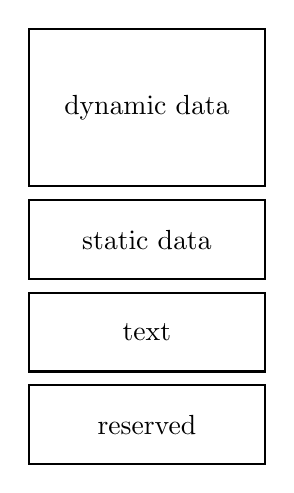
\begin{tikzpicture}[node distance=5pt,nodes={outer sep=0pt,minimum width=3cm, draw, thick, minimum height=1cm}]
      \node (dynamicdata) at (3,2)  [minimum height=2cm] {dynamic data}; 
      \node (staticdata)            [below=of dynamicdata.south] {static data};
      \node (text)                  [below=of staticdata.south] {text};
      \node (reserved)              [below=of text.south] {reserved}; 
    \end{tikzpicture}
  \end{landscape}
\end{document}
